% !TEX root = TexMain.tex
%----------------------------------------------------------------------------------------------------------------------------------------
\chapter{Code Examples of the Core API}\label{sec:codeExamples}
%----------------------------------------------------------------------------------------------------------------------------------------


\section{Data Streams}


In this example we show how to use the main features of a \textit{DataStream} object. More precisely,  we show six different ways of iterating over the data samples of a \textit{DataStream} object.



\begin{lstlisting}
//We can open the data stream using the static class DataStreamLoader
DataStream<DataInstance> data = DataStreamLoader.openFromFile("datasets/SmallDataSet.arff");

//Access to the attributes defining the data set
System.out.println("Attributes defining the data set");
for (Attribute attribute : data.getAttributes()) {
    System.out.println(attribute.getName());
}
Attribute attA = data.getAttributes().getAttributeByName("A");

//1. Iterating over samples using a for loop
System.out.println("1. Iterating over samples using a for loop");
for (DataInstance dataInstance : data) {
    System.out.println("The value of attribute A for the current data instance is: " + dataInstance.getValue(attA));
}


//2. Iterating using streams. We need to restart the data again as a DataStream can only be used once.
System.out.println("2. Iterating using streams.");
data.restart();
data.stream().forEach(dataInstance ->
                System.out.println("The value of attribute A for the current data instance is: " + dataInstance.getValue(attA))
);


//3. Iterating using parallel streams.
System.out.println("3. Iterating using parallel streams.");
data.restart();
data.parallelStream(10).forEach(dataInstance ->
                System.out.println("The value of attribute A for the current data instance is: " + dataInstance.getValue(attA))
);

//4. Iterating over a stream of data batches.
System.out.println("4. Iterating over a stream of data batches.");
data.restart();
data.streamOfBatches(10).forEach(batch -> {
    for (DataInstance dataInstance : batch)
        System.out.println("The value of attribute A for the current data instance is: " + dataInstance.getValue(attA));
});

//5. Iterating over a parallel stream of data batches.
System.out.println("5. Iterating over a parallel stream of data batches.");
data.restart();
data.parallelStreamOfBatches(10).forEach(batch -> {
    for (DataInstance dataInstance : batch)
        System.out.println("The value of attribute A for the current data instance is: " + dataInstance.getValue(attA));
});


//6. Iterating over data batches using a for loop
System.out.println("6. Iterating over data batches using a for loop.");
for (DataOnMemory<DataInstance> batch : data.iterableOverBatches(10)) {
    for (DataInstance dataInstance : batch)
        System.out.println("The value of attribute A for the current data instance is: " + dataInstance.getValue(attA));
}

\end{lstlisting}


\section{Variables}


This example show the basic functionality of the classes Variables and Variable.

\begin{lstlisting}
//We first create an empty Variables object
Variables variables = new Variables();

//We invoke the "new" methods of the object Variables to create new variables.
//Now we create a Gaussian variables
Variable gaussianVar = variables.newGaussianVariable("Gaussian");

//Now we create a Multinomial variable with two states
Variable multinomialVar = variables.newMultionomialVariable("Multinomial", 2);

//Now we create a Multinomial variable with two states: TRUE and FALSE
Variable multinomialVar2 = variables.newMultionomialVariable("Multinomial2", Arrays.asList("TRUE, FALSE"));

//For Multinomial variables we can iterate over their different states
FiniteStateSpace states = multinomialVar2.getStateSpaceType();
states.getStatesNames().forEach(System.out::println);

//Variable objects can also be used, for example, to know if one variable can be set as parent of some other variable
System.out.println("Can a Gaussian variable be parent of Multinomial variable? " +
        (multinomialVar.getDistributionType().isParentCompatible(gaussianVar)));

System.out.println("Can a Multinomial variable be parent of Gaussian variable? " +
        (gaussianVar.getDistributionType().isParentCompatible(multinomialVar)));
\end{lstlisting}



\section{Handling Bayesian Networks}


\subsection{Creating Bayesian Networks with no hidden variables}

In this example, we take a data set, create a BN and we compute the log-likelihood of all the samples
of this data set. The numbers defining the probability distributions of the BN are randomly fixed.

\begin{lstlisting}
//We can open the data stream using the static class DataStreamLoader
DataStream<DataInstance> data = DataStreamLoader.openFromFile("datasets/syntheticData.arff");

/**
 * 1. Once the data is loaded, we create a random variable for each of the attributes 
 * (i.e. data columns) in our data.
 *
 * 2. StaticVariables is the class for doing that. It takes a list of Attributes and 
 * internally creates all the variables. We create the variables using StaticVariables 
 * class to guarantee that each variable has a different ID number and make it 
 * transparent for the user.
 *
 * 3. We can extract the Variable objects by using the method 
 * getVariableByName();
 */
Variables variables = new Variables(data.getAttributes());

Variable a = variables.getVariableByName("A");
Variable b = variables.getVariableByName("B");
Variable c = variables.getVariableByName("C");
Variable d = variables.getVariableByName("D");
Variable e = variables.getVariableByName("E");
Variable g = variables.getVariableByName("G");
Variable h = variables.getVariableByName("H");
Variable i = variables.getVariableByName("I");

/**
 * 1. Once you have defined your StaticVariables object, the next step is to create
 * a DAG structure over this set of variables.
 *
 * 2. To add parents to each variable, we first recover the ParentSet object by the 
 * method getParentSet(Variable var) and then call the method addParent().
 */
DAG dag = new DAG(variables);

dag.getParentSet(e).addParent(a);
dag.getParentSet(e).addParent(b);

dag.getParentSet(h).addParent(a);
dag.getParentSet(h).addParent(b);

dag.getParentSet(i).addParent(a);
dag.getParentSet(i).addParent(b);
dag.getParentSet(i).addParent(c);
dag.getParentSet(i).addParent(d);

dag.getParentSet(g).addParent(c);
dag.getParentSet(g).addParent(d);

/**
 * 1. We first check if the graph contains cycles.
 *
 * 2. We print out the created DAG. We can check that everything is as expected.
 */
if (dag.containCycles()) {
    try {
    } catch (Exception ex) {
        throw new IllegalArgumentException(ex);
    }
}

System.out.println(dag.toString());


/**
 * 1. We now create the Bayesian network from the previous DAG.
 *
 * 2. The BN object is created from the DAG. It automatically looks at the 
 * distribution type of each variable and their parents to initialize the 
 * Distributions objects that are stored inside (i.e. Multinomial, Normal, 
 * CLG, etc). The parameters defining these distributions are properly 
 * initialized.
 *
 * 3. The network is printed and we can have look at the kind of 
 * distributions stored in the BN object.
 */
BayesianNetwork bn = BayesianNetwork.newBayesianNetwork(dag);
System.out.println(bn.toString());


/**
 * 1. We iterate over the data set sample by sample.
 *
 * 2. For each sample or DataInstance object, we compute the log of the probability 
 * that the BN object assigns to this observation.
 *
 * 3. We accumulate these log-probs and finally we print the log-prob of the data set.
 */
double logProb = 0;
for (DataInstance instance : data) {
    logProb += bn.getLogProbabiltyOf(instance);
}
System.out.println(logProb);

BayesianNetworkWriter.saveToFile(bn, "networks/huginStaticBNExample.bn");
\end{lstlisting}


\subsection{Creating Bayesian Networks with hidden variables}

In this example, we simply show how to create a BN model with hidden variables. We simply create a BN for clustering, i.e.,  a naive-Bayes like structure with a single common hidden variable acting as parant of all the observable variables.
 
\begin{lstlisting}

//We can open the data stream using the static class DataStreamLoader
DataStream<DataInstance> data = DataStreamLoader.openFromFile("datasets/syntheticData.arff");

/**
 * 1. Once the data is loaded, we create a random variable for each of the attributes 
 * (i.e. data columns) in our data.
 *
 * 2. StaticVariables is the class for doing that. It takes a list of Attributes and 
 * internally creates all the variables. We create the variables using StaticVariables 
 * class to guarantee that each variable has a different ID number and make it 
 * transparent for the user.
 *
 * 3. We can extract the Variable objects by using the method 
 * getVariableByName();
 */
Variables variables = new Variables(data.getAttributes());

Variable a = variables.getVariableByName("A");
Variable b = variables.getVariableByName("B");
Variable c = variables.getVariableByName("C");
Variable d = variables.getVariableByName("D");
Variable e = variables.getVariableByName("E");
Variable g = variables.getVariableByName("G");
Variable h = variables.getVariableByName("H");
Variable i = variables.getVariableByName("I");

/**
 * 1. We create the hidden variable. For doing that we make use of the class 
 * VariableBuilder. When a variable is created from an Attribute object, it 
 * contains all the information we need (e.g. the name, the type, etc). But 
 * hidden variables does not have an associated attribute and, for this 
 * reason, we use now this VariableBuilder to provide this information to
 * StaticVariables object.
 *
 * 2. Using VariableBuilder, we define a variable called HiddenVar, which is not 
 * observable (i.e. hidden), its state space is a finite set with two elements, 
 * and its distribution type is multinomial.
 *
 * 3. We finally create the hidden variable using the method "newVariable".
 */

Variable hidden = variables.newMultionomialVariable("HiddenVar", Arrays.asList("TRUE", "FALSE"));

/**
 * 1. Once we have defined your StaticVariables object, including the hidden 
 * variable, the next step is to create a DAG structure over this set of variables.
 *
 * 2. To add parents to each variable, we first recover the ParentSet object by 
 * the method getParentSet(Variable var) and then call the method 
 * addParent(Variable var).
 *
 * 3. We just put the hidden variable as parent of all the other variables. Following 
 * a naive-Bayes like structure.
 */
DAG dag = new DAG(variables);

dag.getParentSet(a).addParent(hidden);
dag.getParentSet(b).addParent(hidden);
dag.getParentSet(c).addParent(hidden);
dag.getParentSet(d).addParent(hidden);
dag.getParentSet(e).addParent(hidden);
dag.getParentSet(g).addParent(hidden);
dag.getParentSet(h).addParent(hidden);
dag.getParentSet(i).addParent(hidden);

/**
 * We print the graph to see if is properly created.
 */
System.out.println(dag.toString());

/**
 * 1. We now create the Bayesian network from the previous DAG.
 *
 * 2. The BN object is created from the DAG. It automatically looks at the 
 * distribution type of each variable and their parents to initialize the 
 * Distributions objects that are stored inside (i.e. Multinomial, Normal, 
 * CLG, etc). The parameters defining these distributions are properly 
 * initialized.
 *
 * 3. The network is printed and we can have look at the kind of 
 * distributions stored in the BN object.
 */
BayesianNetwork bn = BayesianNetwork.newBayesianNetwork(dag);
System.out.println(bn.toString());

/**
 * Finally the Bayesian network is saved to a file.
 */
BayesianNetworkWriter.saveToFile(bn, "networks/huginStaticBNHiddenExample.bn");

\end{lstlisting}

\subsection{Modifying Bayesian Networks}

In this example we show how to access and modify the conditional probabilities of a Bayesian network model.

\begin{lstlisting}
//We first generate a Bayesian network with one multinomial, one Gaussian variable and one link
BayesianNetworkGenerator.setNumberOfGaussianVars(1);
BayesianNetworkGenerator.setNumberOfMultinomialVars(1,2);
BayesianNetworkGenerator.setNumberOfLinks(1);

BayesianNetwork bn = BayesianNetworkGenerator.generateBayesianNetwork();

//We print the randomly generated Bayesian networks
System.out.println(bn.toString());

//We first access the variable we are interested in
Variable multiVar = bn.getStaticVariables().getVariableByName("DiscreteVar0");

//Using the above variable we can get the associated distribution and modify it
Multinomial multinomial = bn.getConditionalDistribution(multiVar);
multinomial.setProbabilities(new double[]{0.2, 0.8});

//Same than before but accessing the another variable
Variable normalVar = bn.getStaticVariables().getVariableByName("GaussianVar0");

//In this case, the conditional distribtuion is of the type "Normal given Multinomial Parents"
Normal_MultinomialParents normalMultiDist = bn.getConditionalDistribution(normalVar);
normalMultiDist.getNormal(0).setMean(1.0);
normalMultiDist.getNormal(0).setVariance(1.0);

normalMultiDist.getNormal(1).setMean(0.0);
normalMultiDist.getNormal(1).setVariance(1.0);

//We print modified Bayesian network
System.out.println(bn.toString());

\end{lstlisting}


\section{I/O Functionality}

\subsection{I/O of Data Streams}

In this example we show how to load and save data sets from ".arff" files (http://www.cs.waikato.ac.nz/ml/weka/arff.html)

\begin{lstlisting}
//We can open the data stream using the static class DataStreamLoader
DataStream<DataInstance> data = DataStreamLoader.openFromFile("datasets/syntheticData.arff");

//We can save this data set to a new file using the static class DataStreamWriter
DataStreamWriter.writeDataToFile(data, "datasets/tmp.arff");
\end{lstlisting}

\subsection{I/O of Bayesian Networks}

In this example we show how to load and save Bayesian networks models for a binary file with ".bn" extension. In this toolbox Bayesian networks models are saved as serialized objects.

\begin{lstlisting}
//We can load a Bayesian network using the static class BayesianNetworkLoader
BayesianNetwork bn = BayesianNetworkLoader.loadFromFile("./networks/WasteIncinerator.bn");

//Now we print the loaded model
System.out.println(bn.toString());

//Now we change the parameters of the model
bn.randomInitialization(new Random(0));

//We can save this Bayesian network to using the static class BayesianNetworkWriter
BayesianNetworkWriter.saveToFile(bn, "networks/tmp.bn");
\end{lstlisting}


\section{Inference Algorithms}

\subsection{The Inference Engine}
This example show how to perform inference in a Bayesian network model using the InferenceEngine static class. This class aims to be a straigthfoward way to perform queries over a Bayesian network model. By the default the \textit{VMP} inference method is invoked.

\begin{lstlisting}
//We first load the WasteIncinerator bayesian network which has multinomial 
//and Gaussian variables.
BayesianNetwork bn = BayesianNetworkLoader.loadFromFile("./networks/WasteIncinerator.bn");

//We recover the relevant variables for this example: Mout which is normally 
//distributed, and W which is multinomial.
Variable varMout = bn.getStaticVariables().getVariableByName("Mout");
Variable varW = bn.getStaticVariables().getVariableByName("W");

//Set the evidence.
Assignment assignment = new HashMapAssignment(1);
assignment.setValue(varW,0);

//Then we query the posterior of
System.out.println("P(Mout|W=0) = " + InferenceEngine.getPosterior(varMout, bn, assignment));

//Or some more refined queries
System.out.println("P(0.7<Mout<6.59 | W=0) = " + InferenceEngine.getExpectedValue(varMout, bn, v -> (0.7 < v && v < 6.59) ? 1.0 : 0.0 ));
\end{lstlisting}

\subsection{Variational Message Passing}

This example we show how to perform inference on a general Bayesian network using the Variational Message Passing (VMP)
algorithm detailed in
\vspace{0.2cm}
\textit{Winn, J. M., Bishop, C. M. (2005). Variational message passing. In Journal of Machine Learning Research (pp. 661-694).
}


\begin{lstlisting}
//We first load the WasteIncinerator bayesian network which has multinomial 
//and Gaussian variables.
BayesianNetwork bn = BayesianNetworkLoader.loadFromFile("./networks/WasteIncinerator.bn");

//We recover the relevant variables for this example: Mout which is normally 
//distributed, and W which is multinomial.
Variable varMout = bn.getStaticVariables().getVariableByName("Mout");
Variable varW = bn.getStaticVariables().getVariableByName("W");

//First we create an instance of a inference algorithm. In this case, we use 
//the VMP class.
InferenceAlgorithm inferenceAlgorithm = new VMP();

//Then, we set the BN model
inferenceAlgorithm.setModel(bn);

//If exists, we also set the evidence.
Assignment assignment = new HashMapAssignment(1);
assignment.setValue(varW,0);
inferenceAlgorithm.setEvidence(assignment);

//Then we run inference
inferenceAlgorithm.runInference();

//Then we query the posterior of
System.out.println("P(Mout|W=0) = " + inferenceAlgorithm.getPosterior(varMout));

//Or some more refined queries
System.out.println("P(0.7<Mout<6.59 | W=0) = " + inferenceAlgorithm.getExpectedValue(varMout, v -> (0.7 < v && v < 6.59) ? 1.0 : 0.0 ));

//We can also compute the probability of the evidence
System.out.println("P(W=0) = "+Math.exp(inferenceAlgorithm.getLogProbabilityOfEvidence()));
\end{lstlisting}

\subsection{Importance Sampling}

This example we show how to perform inference on a general Bayesian network using an importance sampling
algorithm detailed in

\vspace{0.2cm}
\textit{Fung, R., Chang, K. C. (2013). Weighing and integrating evidence for stochastic simulation in Bayesian networks. arXiv preprint arXiv:1304.1504.
}

\begin{lstlisting}
//We first load the WasteIncinerator bayesian network which has multinomial 
//and Gaussian variables.
BayesianNetwork bn = BayesianNetworkLoader.loadFromFile("./networks/WasteIncinerator.bn");

//We recover the relevant variables for this example: Mout which is normally 
//distributed, and W which is multinomial.
Variable varMout = bn.getStaticVariables().getVariableByName("Mout");
Variable varW = bn.getStaticVariables().getVariableByName("W");

//First we create an instance of a inference algorithm. In this case, we use 
//the ImportanceSampling class.
InferenceAlgorithm inferenceAlgorithm = new ImportanceSampling();

//Then, we set the BN model
inferenceAlgorithm.setModel(bn);

//If exists, we also set the evidence.
Assignment assignment = new HashMapAssignment(1);
assignment.setValue(varW,0);
inferenceAlgorithm.setEvidence(assignment);

//We can also set to be run in parallel on multicore CPUs
inferenceAlgorithm.setParallelMode(true);

//Then we run inference
inferenceAlgorithm.runInference();

//Then we query the posterior of
System.out.println("P(Mout|W=0) = " + inferenceAlgorithm.getPosterior(varMout));

//Or some more refined queries
System.out.println("P(0.7<Mout<6.59 | W=0) = " + inferenceAlgorithm.getExpectedValue(varMout, v -> (0.7 < v && v < 6.59) ? 1.0 : 0.0 ));

//We can also compute the probability of the evidence
System.out.println("P(W=0) = "+Math.exp(inferenceAlgorithm.getLogProbabilityOfEvidence()));
\end{lstlisting}


\section{Learning Algorithms}

\subsection{Parallel Maximum Likelihood}

This example shows how to learn in parallel the parameters of a Bayesian network from a stream of data using maximum likelihood.
\begin{lstlisting}
//We can open the data stream using the static class DataStreamLoader
DataStream<DataInstance> data = DataStreamLoader.openFromFile("datasets/syntheticData.arff");

//We create a MaximumLikelihood object with the MaximumLikehood builder
MaximumLikelihood parameterLearningAlgorithm = new MaximumLikelihood();

//We activate the parallel mode.
parameterLearningAlgorithm.setParallelMode(true);

//We fix the DAG structure
parameterLearningAlgorithm.setDAG(getNaiveBayesStructure(data,0));

//We set the batch size which will be employed to learn the model in parallel
parameterLearningAlgorithm.setBatchSize(100);

//We set the data which is going to be used for leaning the parameters
parameterLearningAlgorithm.setDataStream(data);


//We perform the learning
parameterLearningAlgorithm.runLearning();

//And we get the model
BayesianNetwork bnModel = parameterLearningAlgorithm.getLearntBayesianNetwork();

//We print the model
System.out.println(bnModel.toString());
\end{lstlisting}

\subsection{Streaming Variational Bayes}

This examples shows how to learn in the parameters of a Bayesian network from a stream of data with a Bayesian
approach using the following algorithm

\textit{Broderick, T., Boyd, N., Wibisono, A., Wilson, A. C., \& Jordan, M. I. (2013). Streaming variational Bayes. 
In Advances in Neural Information Processing Systems (pp. 1727-1735).
}



\subsubsection*{Version 1}

In this first example we show a simple way to invoke this learning algorithm,


\begin{lstlisting}
//We can open the data stream using the static class DataStreamLoader
DataStream<DataInstance> data = DataStreamLoader.openFromFile("datasets/syntheticData.arff");

//We create a StreamingVariationalBayesVMP object
StreamingVariationalBayesVMP parameterLearningAlgorithm = new StreamingVariationalBayesVMP();

//We fix the DAG structure
parameterLearningAlgorithm.setDAG(getHiddenNaiveBayesStructure(data));

//We fix the size of the window, which must be equal to the size of the data batches we use for learning
parameterLearningAlgorithm.setWindowsSize(5);

//We set the data which is going to be used for leaning the parameters
parameterLearningAlgorithm.setDataStream(data);

//We perform the learning
parameterLearningAlgorithm.runLearning();

//And we get the model
BayesianNetwork bnModel = parameterLearningAlgorithm.getLearntBayesianNetwork();

//We print the model
System.out.println(bnModel.toString());
\end{lstlisting}


\subsubsection*{Version 2}

In this second example we show a alternative use of this class which explicitly update the model by batches, 


\begin{lstlisting}
//We can open the data stream using the static class DataStreamLoader
DataStream<DataInstance> data = DataStreamLoader.openFromFile("datasets/syntheticData.arff");

//We create a StreamingVariationalBayesVMP object
StreamingVariationalBayesVMP parameterLearningAlgorithm = new StreamingVariationalBayesVMP();

//We fix the DAG structure
parameterLearningAlgorithm.setDAG(getHiddenNaiveBayesStructure(data));

//We fix the size of the window, which must be equal to the size of the data batches 
//we use for learning
parameterLearningAlgorithm.setWindowsSize(5);


//We should invoke this method before processing any data
parameterLearningAlgorithm.initLearning();


//Then we show how we can perform parameter learnig by a sequential updating of 
//data batches.
for (DataOnMemory<DataInstance> batch : data.iterableOverBatches(5)){
    parameterLearningAlgorithm.updateModel(batch);
}

//And we get the model
BayesianNetwork bnModel = parameterLearningAlgorithm.getLearntBayesianNetwork();

//We print the model
System.out.println(bnModel.toString());
\end{lstlisting}


% !TEX root = TexMain.tex
%----------------------------------------------------------------------------------------------------------------------------------------
\chapter{Code Examples of the HuginLink API}\label{sec:codeExamples}
%----------------------------------------------------------------------------------------------------------------------------------------

\section{Models conversion between AMIDST and Hugin}

This example shows how to use the class BNConverterToAMIDST and BNConverterToHugin to convert a 
Bayesian network models between Hugin and AMIDST formats


\begin{lstlisting}
//We load from Hugin format
Domain huginBN = BNLoaderFromHugin.loadFromFile("networks/asia.net");

//Then, it is converted to AMIDST BayesianNetwork object
BayesianNetwork amidstBN = BNConverterToAMIDST.convertToAmidst(huginBN);

//Then, it is converted to Hugin Bayesian Network object
huginBN = BNConverterToHugin.convertToHugin(amidstBN);

System.out.println(amidstBN.toString());
System.out.println(huginBN.toString());
\end{lstlisting}



\section{I/O of Bayesian Networks}

This example shows how to use the class BNLoaderFromHugin and BNWriterToHugin classes to load and
write Bayesian networks in Hugin format.

\begin{lstlisting}
//We load from Hugin format
Domain huginBN = BNLoaderFromHugin.loadFromFile("networks/asia.net");

//We save a AMIDST BN to Hugin format
BayesianNetwork amidstBN = BNConverterToAMIDST.convertToAmidst(huginBN);
BNWriterToHugin.saveToHuginFile(amidstBN,"networks/tmp.net");
\end{lstlisting}

\section{Invoking Hugin's inference engine}

This example we show how to perform inference using Hugin (http://www.hugin.com) inference engine within the AMIDST toolbox

\begin{lstlisting}
//We first load the WasteIncinerator bayesian network which has multinomial and Gaussian variables.
BayesianNetwork bn = BayesianNetworkLoader.loadFromFile("./networks/WasteIncinerator.bn");

//We recover the relevant variables for this example: Mout which is normally distributed, and W which is multinomial.
Variable varMout = bn.getStaticVariables().getVariableByName("Mout");
Variable varW = bn.getStaticVariables().getVariableByName("W");

//First we create an instance of a inference algorithm. In this case, we use the ImportanceSampling class.
InferenceAlgorithm inferenceAlgorithm = new HuginInference();
//Then, we set the BN model
inferenceAlgorithm.setModel(bn);

//If exists, we also set the evidence.
Assignment assignment = new HashMapAssignment(1);
assignment.setValue(varW,0);
inferenceAlgorithm.setEvidence(assignment);

//Then we run inference
inferenceAlgorithm.runInference();

//Then we query the posterior of
System.out.println("P(Mout|W=0) = " + inferenceAlgorithm.getPosterior(varMout));

//Or some more refined queries
System.out.println("P(0.7<Mout<3.5 | W=0) = " + inferenceAlgorithm.getExpectedValue(varMout, v -> (0.7 < v && v < 3.5) ? 1.0 : 0.0 ));

\end{lstlisting}

%%% Local Variables:
%%% mode: latex
%%% TeX-master: "TexMain"
%%% End:

\begin{lstlisting}


\end{lstlisting}

% !TEX root = TexMain.tex
%----------------------------------------------------------------------------------------------------------------------------------------
\chapter{MoaLink Module: AMIDST models from MOA}\label{sec:codeExamples}
%----------------------------------------------------------------------------------------------------------------------------------------

\section{Generate Jar with AMIDST extension}
In the moalink directory, run the \texttt{compileWithDependencies.sh}. A moalink-1.0-SNAPSHOT-jar-with-dependencies.jar will be generated in the \texttt{target} directory. Please place this jar file on your library path for moa. 

With this jar file we can make use of the different learning and inference algorithms in AMIDST to learn for expressive Bayesian network models for classification, regression and clustering. AMIDST offer the possibility to add latent Gaussian and/or Multinomial variables to a base naive Bayes structure. Normally, the addition of these latent variables should provide classifiers with lower bias and higher variance, that is, more sophisticated classifiers that are able to lean more complex interdependencies in the data but also more prone to overfit. The user should evaluate the complexity of his/her dataset and choose the number of latent Gaussian variables and states of the multinomial latent variable accordingly.

With the following command, MOA gui can be invoked e.g (remember to place \texttt{compileWithDependencies.sh} under the lib folder reference in the \verb'-cp' option):

\begin{verbatim}
java -Xmx512m -cp "../lib/*" -javaagent:../lib/sizeofag-1.0.0.jar
moa.gui.GUI
\end{verbatim}

In the following sections we include some command examples to use the AMIDST models from MOA from the command line in a Unix machine\footnote{Note that these examples should be slightly adapted to run on a Windows machine: e.g. use \textasciicircum~ instead of \textbackslash~ to escape brackets.}.

\section{AMIDST Classifiers from MOA}

The following command can be used to learn a Bayesian model with a latent Gaussian variable (HG) and a multinomial with 2 states (HM), as displayed in Figure \ref{fig:HODE} (a). The VMP algorithm is used to learn the parameters of these two non-observed variables and make predictions over the class variable.

\begin{figure}[htb]
   \centering
   \begin{tabular}{cc}
	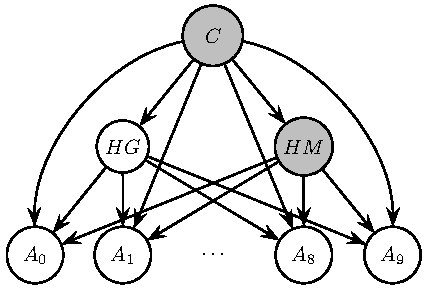
\includegraphics[scale=0.8]{figs/HODE}&
	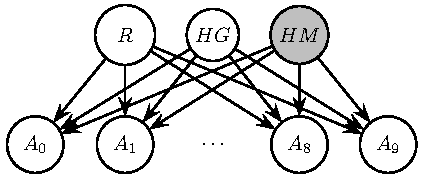
\includegraphics[scale=0.8]{figs/regressionHODE}\\
	(a) Model for classification & (b) Model for regression \\
	\end{tabular}
\caption{Bayesian network model learnt for a stream of data with $10$ numeric attributes. Grey nodes represent discrete variables and white nodes continuous variables. It corresponds to a Naive Bayes model structure enriched with a Gaussian and a 2-state multinomial parent. The C and R variables represent the class and the regressor variables respectively.}
\label{fig:HODE}
\end{figure}

\begin{verbatim}
java -Xmx512m -cp "../lib/*" -javaagent:../lib/sizeofag-1.0.0.jar 
moa.DoTask EvaluatePrequential -l \(bayes.AmidstClassifier -g 1 
-m 2\) -s generators.RandomRBFGenerator -i 10000 -f 1000 -q 1000
\end{verbatim}

\section{AMIDST Regression from MOA}

It is possible to learn an enriched naive Bayes model for regression if the class label is of a continuous nature. The following command uses the model in Figure \ref{fig:HODE}(b) on a toy dataset from WEKA's collection of regression problems\footnote{\url{http://prdownloads.sourceforge.net/weka/datasets-numeric.jar}}.

\begin{verbatim}
java -Xmx512m -cp "../lib/*" -javaagent:../lib/sizeofag-1.0.0.jar 
moa.DoTask EvaluatePrequentialRegression -l bayes.AmidstRegressor
 -s (ArffFileStream -f ./quake.arff)
\end{verbatim}

Note that the simpler the dataset the less complex the model should be. In this case, \texttt{quake.arff} is a very simple and small dataset that should probably be learn with a more simple classifier, that is, a high-bias-low-variance classifier, in order to avoid overfitting. This aims at providing a simple running example.

%\section{AMIDST Clustering from MOA}